\colorbox{white!10!}{
    \begin{minipage}{0.2\textwidth}
       \begin{flushleft}
        
\includegraphics[width = 0.6\textwidth]{Эмблема.png}
       \end{flushleft}
    \end{minipage}
    \begin{minipage}[t]{0.7 \textwidth}
        \begin{center}
            {\huge \textsc{Красноярская Летняя Школа. Сезон $7^2 - 2$}}
            \vspace{0.25cm}
            
            { \huge \textbf{ФМТ. Тур 4.2}}
        \end{center}
        \vspace{0.05cm}
    \end{minipage}
}

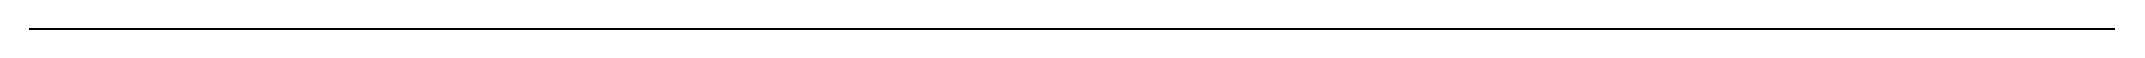
\begin{tikzpicture}
    \draw[thick] (-6.5,0)--(20,0);
\end{tikzpicture}
\begin{enumerate}
    \item Пассажир поезда заметил, что проехал по мосту за 20 с. Часовой, охраняющий мост, зарегистрировал, что поезд находился на мосту 70 с. Во сколько раз длина поезда больше длины моста?
	\item В калориметр с $\tau = 200$ г воды при температуре $t_0 = 60^{o}C$  поместили три кубика льда массой $m = 10$ г каждый, имеющие температуры $t_1 = -10^{o}C$, $t_2 = -20^{o} C$ и $t_3 = -30^{o} C$. Какая температура установится в калориметре? Удельная теплота плавления льда $\lambda = 330 \frac{\text{кДж}}{\text{кг}}$, удельные теплоёмкости воды и льда соответственно $c_{\text{в}} = 4200 \frac{\text{Дж}}{\text{кг\ C}}$ и $c_{\text{л}} = 2100 \frac{\text{Дж}}{\text{кг\ C}}$.  

\end{enumerate}